\section{PIA}
La PIA è un dispositivo di comunicazione parallela ad 8 bit. Tale architettura è un dispositivo hardware che si posiziona tra la periferica e il processore stesso. Essa è costituita architetturalmente da due tipologie diverse di porto, il porto A ed il porto B.[\ref{img:PIA}]
Tali porti hanno dei registri che sono direzionali, quindi possono assumere una sola funzione (tra entrata ed uscita), in base alla loro specifica impostazione e configurazione.
Prima di parlare di più porti ci concentriamo sulle comunicazioni a singolo porto; in generale le comunicazioni che avvengono tra due interfacce della PIA utilizzano il protocollo di handshacking. Entrando nei dettagli del processo, bisognerà fare particolare attenzione ai seguenti registri:
\begin{itemize}
    \item \textbf{CA1,CB1}: Sono registri che possono assumere solo direzione di ingresso e solitamente vengono usati come "lettori" di segnali SYN o segnali ACK da parte dell'altro dispositivo
    \item \textbf{CA2,CB2}: Sono i registri che possono essere configurati(sia di ingresso che di uscita), ed in generale, in base al protocollo che si vuole interpretare, vengono settati in una determinata modalità di funzionamento (dipendente dalla tipologia di protocollo che si vuole implementare)
    \item \textbf{Dato}: Il bus dati trasmette parallelamente i dati tra le due periferiche in base al protocollo di handshacking utilizzato
\end{itemize}

\begin{figure}
    \centering
    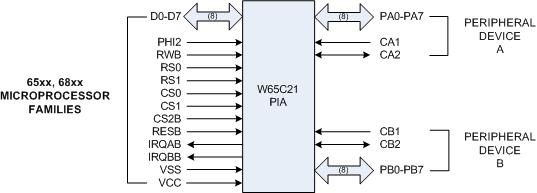
\includegraphics[width=.6\textwidth]{img/PIA.png}
    \caption{Architettura base della PIA}\label{img:PIA}
\end{figure}


\begin{figure}
    \centering
    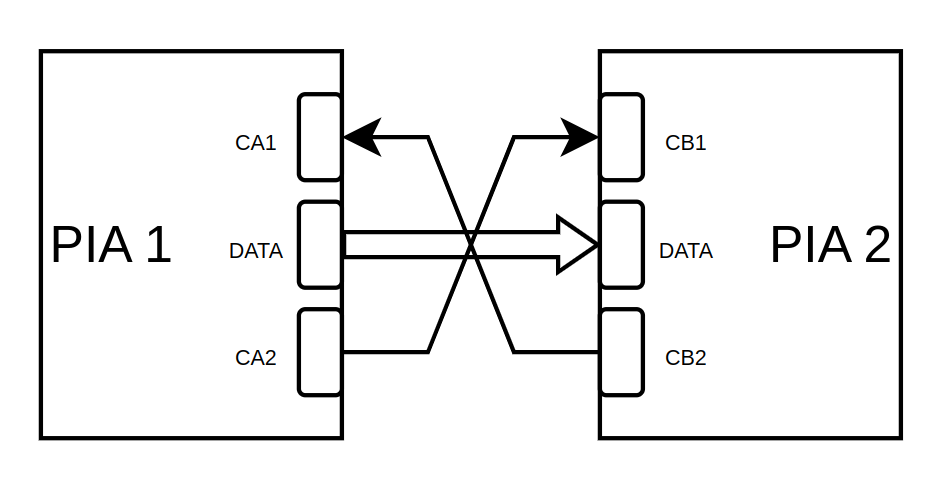
\includegraphics[width=0.65\textwidth]{img/PIA-CON.png}
    \caption{Collegamento tra due dispositivi tramite PIA}\label{img:PIA-CON}
\end{figure}
Per far di che le due architetture possano comunicare è quindi importante definire come si andranno a collegare e quindi la direzione e l'interpretazione che devo andare a dare ai registri. Una possibile architettura di collegamento è quella visibile all'immagine [\ref{img:PIA-CON}].
Una volta definita la tipologia di architettura si va a decidere come queste periferiche dovranno interagire tra loro (definizione del protocollo o modello di programmazione della PIA)